\documentclass[a4paper,10pt]{article}
\usepackage[utf8]{inputenc}
\usepackage[margin=3cm]{geometry}
\usepackage{amsmath}
\usepackage{amssymb}
\usepackage{amsthm}
\usepackage{fancyhdr}
\usepackage{seminar}
\usepackage{graphicx}
\usepackage{subfigure}
\usepackage{float}
\usepackage{listings}
\usepackage{hyperref}

\pagestyle{fancy}


%You can add theorem-like environments (e.g. remark, definition, ...) if you want
\newtheorem{theorem}{Theorem}

\title{Isospectralization}
\author{Sricharan Chiruvolu} % Replace with your name
\institute{Department of Informatics - Technische Universit\"{a}t M\"{u}nchen} % Replace with the department you belong to

\makeatletter
\let\runauthor\@author
\let\runtitle\@title
\makeatother
\lhead{\runauthor}
\rhead{\runtitle}




\begin{document}

\maketitle

\begin{abstract}

This report discusses the technique of \texttt{isospectralization} or ``Can you hear the shape, style, and correspondence of a drum?", a numerical optimization procedure to deform a mesh in order to align its (finite) Laplacian spectrum with a given one. Based on the CVPR 2019 paper of the same name \cite{cosmo2018isospectralization}, the report explores the practical possibility of using the spectrum of an object for shape reconstruction and the applications of such a technique.

\end{abstract}

\section{Introduction}

Mark Kac’s 1966 question, ``Can one hear the shape of a drum?" \cite{kac1966can}
set off research into spectral theory, with the idea of understanding
the extent to which the spectrum allows one to read back the
geometry. If such recovery is possible through its Laplacian spectrum
is a classical problem explored over the past few decades. Although theoretically negative, in practice we can approximate the solution (Figure \ref{fig:Isospectralization}). This problem is highly non-linear and thus particularly difficult, making it susceptible to local minima.

This paper explores one such numerical optimization technique, isospectralization. We will introduce mathematical background, formal problem description, the algorithm and potential applications for this problem. We also emphasis our discussion on the proposed inverse mapping between geometric domain and its Laplacian via  regularizers.

\begin{figure}[hbt!]
    \centering
    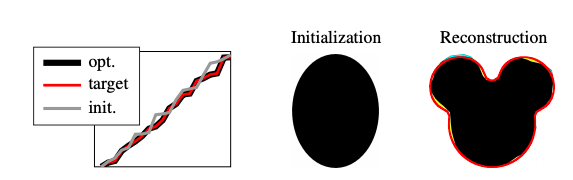
\includegraphics[height=0.2\textwidth]{Spectral.png}
    \caption{Isospectralization}
    \label{fig:Isospectralization}
\end{figure}



\section{Background}

Spectral geometry is the study of the relationships between geometric properties of the manifold and properties of its spectrum.

The Notion of spectrum is an essential part in various fields including classical mechanics, quantum mechanics, analysis, and of course, geometry that we'd discuss more here. Both quantum physics and general relativity also try to drive through the spectral approach - Can one hear the shape of the universe?

In this section, we'll start with the basic idea of a (Riemannian) manifold and the Laplace-Beltrami operator.


\begin{figure}[hbt!]
 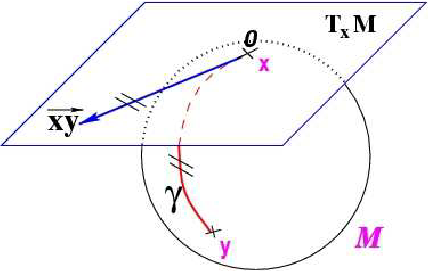
\includegraphics[height=0.3\textwidth]{Geodesics2.png}
 \centering
 \caption{\label{fig:Geodesics}Geodesic and tangent space in a Riemannian manifold. \cite{berger2006panoramic}}
\end{figure}

\subsection{Riemannian manifolds}

A manifold is defined as a topological space that locally resembles Euclidean space near each point. This notion allows complicated systems to be explained in simpler terms of local topological properties of Euclidean space.


In computer vision, the notion a manifold is used quite frequently -- in rotation averaging ($ SO3 $), structure and motion ("Essential" manifold), to capture the shape of an object ("Shape" manifolds), to model a set of images ("Grassman" manifolds) or to simply represent a sphere ($ S^n $).

A "Hilbert" space is an abstract vector space with an inner product which has to be complete under convergence (i.e. to allow calculus to be used). This generalises the notion of Euclidean space by extending the methods of vector algebra and calculus from 2D Euclidean plane and 3D spaces to higher dimensions. Thus, we can define norms in Hilbert space to allow us to measure distances, and inner products to allow us to measure angles.

On a Riemannian manifold (Figure \ref{fig:Geodesics}), you get to measure lengths of the curves. A Riemannian manifold is a manifold with an inner product defined in the tangent space at each point. A Riemannian metric (tensor) makes it possible to define several geometric notions on a Riemannian manifold, such as angle at an intersection, length of a curve, area of a surface and higher-dimensional analogues (volume, etc.), extrinsic curvature of submanifolds, and intrinsic curvature of the manifold itself. It also allows us to define "geodesic distance" on the manifold.

Geodesics are locally shortest curves. They preserve a direction on a surface and have many interesting properties. In a plane, the geodesics are straight lines. On a sphere, the geodesics are great circles (like the equator). The geodesics in a space depend on the Riemannian metric, which affects the notions of distance and acceleration. Again, metric geometry is a field by itself.

Equivalently in other areas, it can be defined as a path that a particle which is not accelerating would follow.

In Riemannian geometry, all geodesics are locally distance-minimizing paths, but the converse is not true.

\subsection{Isometry and Isomorphism}


An isometry (Figure \ref{fig:isometry}) of a manifold can be defined as any (smooth) mapping of that manifold (into itself, or into another manifold) that preserves the notion of distance between points.

When such a mapping is on smooth manifolds (and is a diffeomorphism: the mapping is a bijection and its inverse is differentiable), it is called isometry, and provides a notion of isomorphism ("sameness").


\textbf{Notation}: Let $ M $ be a smooth manifold. Denote the tangent space at $ x \in M $ by $ T_{x}M $.

If $ f:M \xrightarrow{} N $ is a smooth map between smooth manifolds, denote the associated map on $ T_{x}M $ by $ (Df){x}:T{x}M \xrightarrow{} T_{f(x)}N $. If $ I $ is an open interval in $ \mathbb{R} $ and $ \alpha : I \xrightarrow{} M $ is a smooth path, then for $ t \in I, \alpha` (t) $ denotes $ (D \alpha)_{t}(I) \in T_{\alpha(t)}M $.

\textbf{Definition} : A Riemannian metric on a smooth manifold M is a choice at each point $ x \in M $ of a positive definite inner product $ <, > $ on $ T_{x}M $, the inner products varying smoothly with $ x $. Then $ M $ is known as a Riemannian manifold.

\begin{theorem}

A local isometry between two Riemannian manifolds $ M $ and $ N $ is a local diffeomorphism $ h: M \xrightarrow{} N $, such that, for all points $ x \in M $ and all vectors $ v $ and $ w $ in $ T_{x}M $ is denoted by,

\begin{equation}
 <v, w> =  <(Dh)_{x}(v), (Dh)_{x}(w)>
\end{equation}
A (Riemannian) isometry is a local isometry that is also a diffeomorphism.
\end{theorem}

\begin{figure}[hbt!]
    \centering
    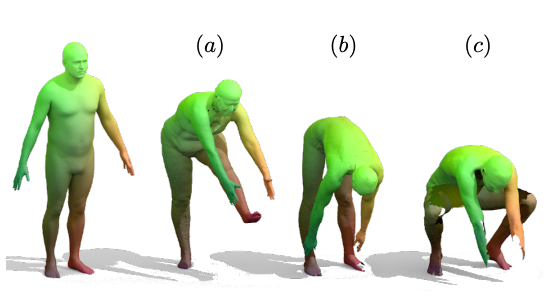
\includegraphics[height=0.4\textwidth]{isometry.png}
    \caption{Isometry and Isomorphism. The surfaces are isometric to each other, and the color corresponds to the correpondences.}
    \label{fig:isometry}
\end{figure}


\subsection{Laplace-Beltrami Operator}

\begin{figure}
    \centering
    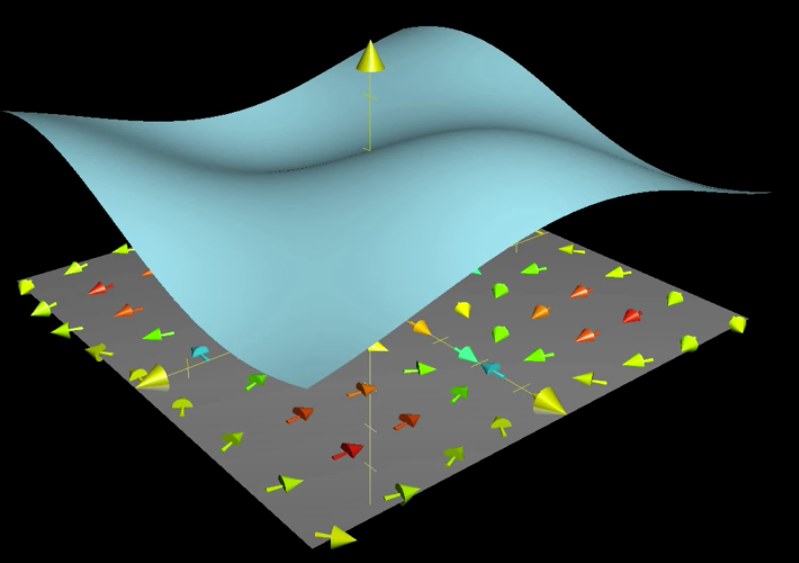
\includegraphics[width=0.4\textwidth]{laplacian.png}
    \caption{Laplace-Beltrami operator. The projected plane shows the curls and gradients of the manifold. The operator is analogous to second gradient. Image from \cite{eisenberger2019smooth}.}
    \label{fig:laplacian}
\end{figure}

The Laplace operator is a fundamental concept in calculus, given by the divergence of the gradient of a function on Euclidean space. The laplacian of a function $ f $ at point $ p $ is the rate at which the average value of $ f $ over spheres centered at $ p $ deviates from $ f(p) $ as the radius of the sphere shrinks towards 0.

Initially introduced in the study of celestial mechanics, solutions of the equation $ \triangle f = 0 $, now called Laplace's equation, are the so-called harmonic functions and represent the possible gravitational fields in regions of vacuum.

The Laplacian generalized to the Riemannian manifold $ (M,g) $ by the Laplace-Beltrami operator ($ {\triangle}_g $) (Figure \ref{fig:laplacian}). 

Equivalently other areas (esp. in diffusion processes) utilize this idea - Fluid mechanics (the Navier-stokes equation), potential theory (Poisson equation), heat diffusion (heat equation), wave equation, quantum physics (Schrodinger equation) and so on.

\subsection{Spectral Geometry}

Spectral geometry is a field in mathematics which concerns relationships between geometric structures of manifolds and spectra of canonically defined differential operators.

Given a compact Riemannian manifold, we can associate to it the (linear unbounded) Laplace-Beltrami operator. This operator is self-adjoint and its spectrum is discrete : namely the spectrum consists of a increasing sequence of real eigenvalues with finite multiplicity.

Two closed Riemannian manifolds are said to be isospectral if the eigenvalues of their Laplace Beltrami operator (Laplacians), counted multiplicities, coincide.

Thus, spectral geometry is the connection between the spectrum $ Spec(M; g) $ and the geometry of the manifold $ (M; g) $ \cite{Yiaza}. This fundamentally deals with two kinds of problems:

\subsection{Direct Problems}

A problem that arises a lot in physics, the analysis of PDEs, probability etc is to compute the spectrum of Laplacian (or other operators). The main idea is to find a lower bound estimate on the eigenvalues of the spectrum on a Riemannian manifold. This is we,

\textit{Compute (exactly or not) the spectrum $ Spec(M, g) $? And (or) find properties on the spectrum $ Spec(M,g) $?}

Direct problems attempt to infer the behavior of the eigenvalues of a Riemannian manifold from knowledge of the geometry.

\subsection{Inverse Problems}

One of fundamental problems in spectral geometry is to ask to what extent the eigenvalues determine the geometry of a given manifold.

If the notion that a Riemannian invariant is true: if two Riemannian manifolds $  (M; g) $ and $ (M', g') $ are isometric, then they are isospectral i.e., $ Spec(M, g) == Spec(M', g') $?

\textit{Does the data of the spectrum $ Spec(M, g) $ determine the ``shape" of the manifold $ (M, g) $?}

This question of isospectrality (spectral alignment) in Riemannian geometry may be traced back to H. Weyl in 1911–1912 and became popularized thanks to M. Kac’s article of 1966. The famous sentence of Kac “Can one hear the shape of a drum?” refers to this type of isospectral problem.

\section{Isospectralization}

\begin{figure}[hbt!]
 \includegraphics[width=\textwidth]{notations}
 \caption{\label{fig:notations}Notations}
\end{figure}

\subsection{Notations}

In the discrete setting, one shape can be approximated by manifold triangle meshes $ X = (V, E, F) $,
where $ V $ is the set of vertices sampled at $ v1, ..., vn $, and where each edge $ eij \in Ei  \cap Eb $ belongs
to at most two triangle faces $Fijk$ and $Fjih$, as shown in figure. The discrete metric is defined by assigning a length $lij > 0$
 to each edge $eij \in E$ (Figure \ref{fig:notations}).
 
  The discrete Laplace-Beltrami operator is defined in the form of a n by n matrix $\triangle = A^{-1}W$, where A
is a diagonal matrix of local area elements, and W is a symmetric matrix of
edge-wise weights.

\subsection{Optimization}

\begin{theorem}
Isospectralization: the optimal embedding that aligns the spectrum to another when $\mathbf{V}$ is the (unknown) embedding of the mesh vertices in $\mathbb{R}$ and $\boldsymbol{\Delta}_{X}(\mathbf{V})$ is the associated discrete Laplacian is defined as,

\begin{equation}
\min _{\mathbf{V} \in \mathbb{R}^{n \times d}}\left\|\boldsymbol{\lambda}\left(\boldsymbol{\Delta}_{X}(\mathbf{V})\right)-\boldsymbol{\mu}\right\|_{\omega}+\rho_{X}(\mathbf{V}) 
\end{equation}

where $\rho_{X}(\mathbf{V})$ are the associated regularization factors of the shape in $\mathbb{R}$.
\end{theorem}

A weighted norm is applied rather than an l2-norm because to make the error diffusion from  the high end of the spectrum that accounts for small geometric variations of the embedding more balanced.

\begin{figure}[hbt!]
 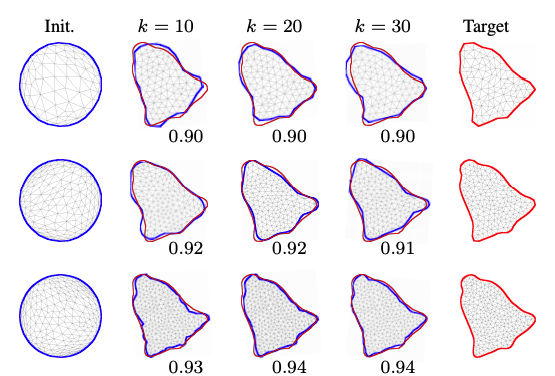
\includegraphics[height=0.5\textwidth,keepaspectratio]{Flatshapes}
 \centering
 \caption{\label{fig:Flatshapes} Shape recovery optimization for flat shapes.}
\end{figure}

\subsection{Flat Shape Regularizers}

In $ \mathbb{R}^2 $ the shape can be optimized by emphasising on the boundary of the shape. Thus the boundary vertices play a more vital role. Three kinds of regularizers can be applied on the surfaces in this case. The first one is to encourage smaller boundary edge lengths by penalising longer perimeters by the summation of the edge vertices. 


    \begin{equation}
           \rho_{X}(\mathbf{V}) = \sum_{e_{ij} \in E_{b}} l_{ij}(\mathbf{V}) 
    \end{equation}  
 
This is called the Tikhonov regularizer and it promotes short
edge lengths and thus a uniformly sized mesh.

A second term penalizes triangle flips that may
occur throughout the optimization, and works under the assumption of clockwise oriented triangles. Whenever a triangle flip occurs, the regularizer value increases quadratically. 
  
    \begin{equation}
    \rho_{X}(V)=\left(\min \left(0, r_{X}(V)\right)\right)^{2}
    \end{equation}
   
   \begin{equation}
   r_{X}(V)=\sum_{i j k \in F}\left(R \pi / 2 \left(\mathbf{v}^{j}-\mathbf{v}^{i}\right)\right)^{T}\left(\mathbf{v}^{k}-\mathbf{v}^{i}\right)
   \end{equation}
  
The final regularizer makes sure that the internal edges are uniform, by applying an l2-norm over all internal edge lengths.

    \begin{equation}
     \rho_{X}(\mathbf{V}) = \sum_{e_{ij} \in E_{i}} l_{ij}^2(\mathbf{V})
    \end{equation}

The summation of these regularizers are applied to penalize the optimization equation.


\subsection{Effects of Regularizers}


The reconstruction quality is measured as
the area ratio of the intersection of the recovered and target embeddings over their union (IOU, the higher the better) after an optimal alignment has been carried out (Figure \ref{fig:Flatshapes}).

The other hyperparameters include the mesh resolution and the bandwidth (chosen eigenvalue sequence). It is observed that higher number of meshes significantly improves reconstruction quality. Same goes for the bandwidth except that choosing over 30 eigenvalues does not increase the reconstruction quality anymore.

\subsection{Surface Regularizers}

For high dimensional surfaces, different regulaizers are proposed. This is in particular because the volume of the surface plays more importance than the outer edges (if any). 

The first regularizer makes sure that the vertex is equidistant from its boundary vertices, thereby optimizing for a uniformly sized mesh. This done with the graph Laplacian and encouraging vertices to lie close to the barycenter of the neighbours. 

    \begin{equation}
 \rho_{X}(\mathbf{V}) = \left\| \mathbf{L}_0^g \mathbf{V}  \right\|_{2}^{2}
    \end{equation}
    
Here $L$ is the graph Laplacian of the initial embedding.
This term has the effect of promoting both a smooth surface
and a more uniformly sampled embedding.

The second regularizer encourages small total displacement from initial embedding. This would help the volume of the mesh to grow/shrink to disambiguate between isometric shapes (Figure \ref{fig:Surfaces}).

    \begin{equation}
    \rho_{X}(\mathbf{V})=\sum_{i=1}^{n}\left(a_{i}\left(\mathbf{v}^{i}-\mathbf{v}_{0}^{i}\right)\right)^{2}
    \end{equation}


\begin{figure}
 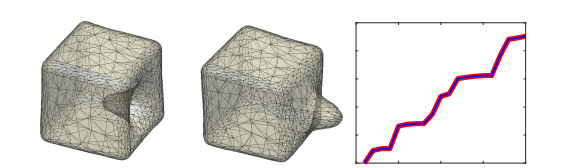
\includegraphics[width=\textwidth]{Surfaces}
 \caption{\label{fig:Surfaces} Two isometric shapes (``Surfaces") with different volume; their (identical) spectra. This is the reason we need the second regularizer to disambiguate isometric shapes.}
\end{figure}


\subsection{Implementation}

Modern deep learning libraries can be employed for this optimization esp. the autodiff capabilities.

However, isospectralization has no
guarantee to reach a (local or global) optimum.

An example PyTorch code for the flat shape regularizer looks would look like this: 

\begin{lstlisting}[language=Python]
 # Inner points regularizer
varA = torch.std(Ak, dim=[0])
inner_reg_cost = params.inner_reg * (l2_loss(L) + l2_loss(varA))

# Boundary points regularizer
bound_reg_cost = params.bound_reg * decay \
* torch.sum(L[bound_edges[:, 0], :])
\end{lstlisting}

For flat shapes, the regularizer for internal edges and the boundaries are applied in a cyclic manner. Triangulation is done after every few steps for more uniform meshes.

\section{Results/ Applications}

The hypothesis of isospectralization is applied on a couple of 
the problems, finding correspondences between non-rigid
shapes and style transfer.

\subsection{Non-isometric shape matching}

The idea is that the alignment of the
spectra of two shapes can make them more intrinsically isometric, and thus can facilitate finding accurate correspondences using existing techniques. This can be easily applied to a sub-class of non-rigid
shape deformations - intrinsic isometries \cite{kim2011blended}, in which the underlying map is assumed to approximately preserve geodesic distances between pairs of points on the shapes (Figure \ref{fig:Correspondenses}). 

\begin{figure}[hbt!]
 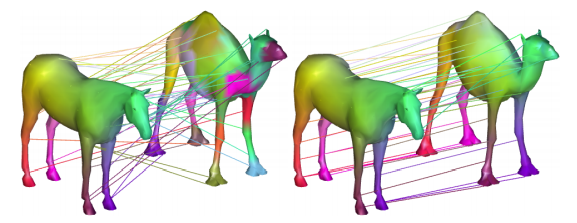
\includegraphics[width=\textwidth]{Correspondenses.png}
 \caption{\label{fig:Correspondenses} Isospectralization as pre-processing for dense correspondence matching. Right: with Isospectralization. Left: without Isospectralization.}
\end{figure}

Isospectralization implements
a notion of correspondence-free alignment, as
it does not require a map between them, of the functional spaces spanned by the first k Laplacian eigen functions. Although a lot of counterexamples of this alignment exists, in most practical cases, this prepossessing step seems to be useful in establishing correspondences for example via \cite{ovsjanikov2016computing}.


\subsection{Style Transfer}
\begin{figure}[hbt!]
    \centering
    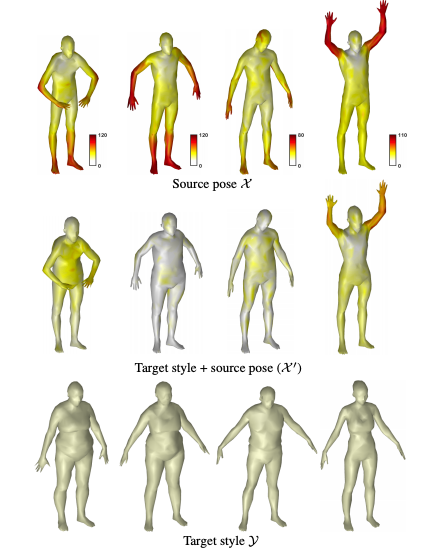
\includegraphics[height=0.5\textwidth]{Styletransfer.png}
    \caption{Isospectralization for Style Transfer. Style is transfered from row 1 to match with row 3. Color shows geodesic error.}
    \label{fig:styletransfer}
\end{figure}

The same idea can also be applied for transferring style between deformable surfaces (Figure \ref{fig:styletransfer}). We can transfer the geometric details of a shape in a certain pose to the shape in another without establishing correspondences and directly by aligning their spectra.

\section{Conclusion}

Isospectralization shows improvement for modern shape matching problems via addressing a decades old problem of "hearing the shape of drum". 

This idea has applications in various domains of geometry processing and computer vision. The mathematical proof that the optimization converges (with the help of regularizers) to the local minimal does not exist yet. There is also no experimental proof of shape interpolation via isospectralization. Nevertheless, the idea has tremendous potential.

\newpage
\bibliographystyle{plain}
\bibliography{egbib}
\end{document}
